\chapter{Methods for Learning from SITS Data}
\label{chapter:meth_model}

\begin{figure}[ht!]
    \centering
    \caption{Graphical abstract showing the whole training and inference stages.}
    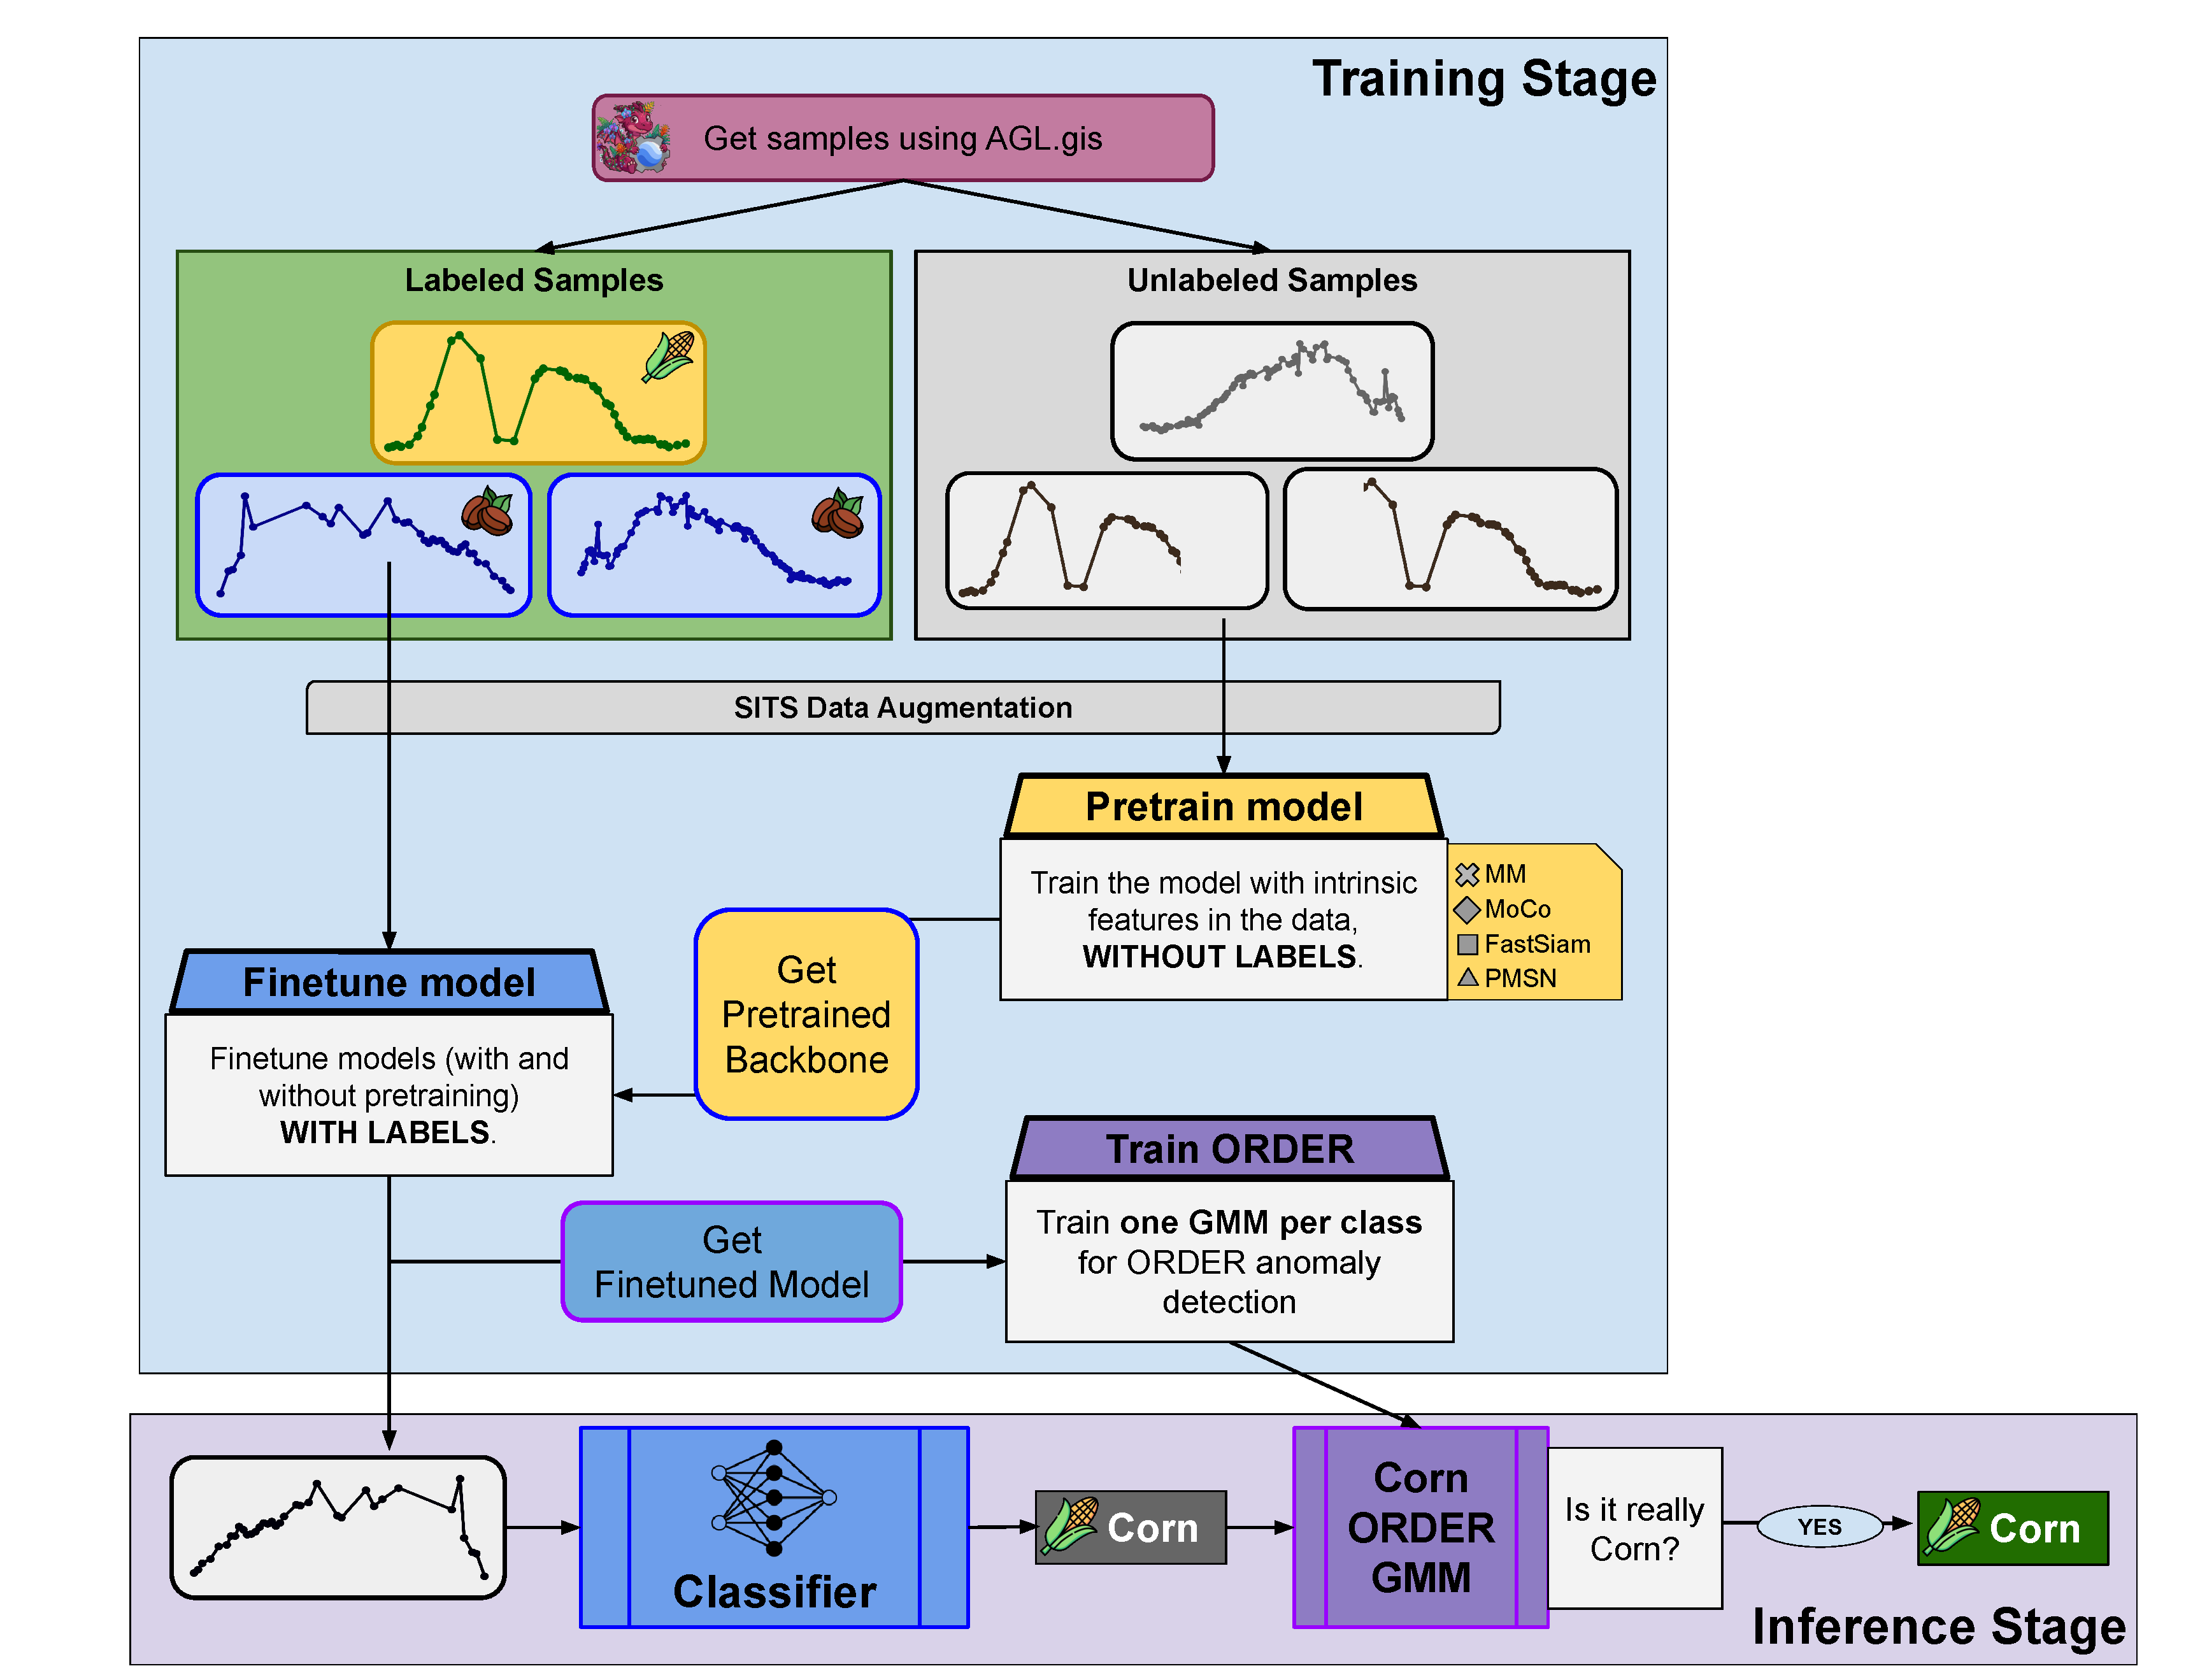
\includegraphics[width=1\linewidth]{figures/6_methodology/meth_graphical_abstract.pdf}
    \label{fig:meth_graphical_abstract}
\end{figure}

With the dataset already consolidated and the samples downloaded using what was presented in the previous chapter (see \autoref{chapter:meth_data}), this pipeline (see \autoref{fig:meth_graphical_abstract}) begins by differentiating between labeled and unlabeled samples (in this work, the unlabeled samples are the same as the labeled ones, but always using all the samples in the dataset). Both undergo a data augmentation process, and the unlabeled samples are used as pre-training for the model. With the trained model backbone, the labeled samples are used for fine-tuning, creating a model capable of classifying predictions. Finally, a \ac{GMM} per class is trained for the \ac{ORDER} method of anomaly detection. In the inference stage, a new sample is received and classified. It receives a class, and the GMM specific to that predicted class checks if there was an anomaly in the model or not. If not, the prediction is confirmed. This pipeline is explained in detail in this chapter.

To establish a robust baseline for \ac{DL} models, this work implemented \ac{SL}-based methodologies. Although \ac{DL} models operate directly on raw data, traditional algorithms require a preliminary feature engineering step to transform the temporal dimension into a structured tabular format, since \ac{SL} models do not handle data of varying sizes.

The preprocessing strategy adopted for \ac{SL} models consisted of reducing the temporal dimensionality by calculating monthly averages. As defined in the implemented transformation pipeline, the time series, originally composed of sequences of \ac{DoY}s and spectral bands, were resampled to 12 fixed time steps (one per month), where the values of each band were aggregated. The resulting vector for each sample was then normalized and flattened to serve as input to the classifiers.

Four SL models were evaluated: RF, SVM, GB through the LGBM library, and an MLP. However, it is known that the process of choosing/creating the best features is time-consuming and often impractical. Therefore, the literature is shifting towards DL models, due to their ability to also learn features.


\section{Deep Architectures for SITS Modeling}
\label{sec:models_supervised}

To evaluate the performance of different paradigms of DL models in SITS crop classification, this work implemented five distinct architectures. These range from attention-based models (Transformers) to recurrent, convolutional, and post-Transformer approaches. All networks share a common input structure, where time series of satellite images are processed to generate embeddings that feed a final linear classifier.

\noindent{\textbf{SITS-CNN:}} To evaluate the performance of convolutional networks, SITS-ConvNeXt was designed, based on the modern ConvNeXt CNN. This architecture adapts the blocks of the ConvNeXt network, originally designed for 2D computer vision, to handle SITS. The implementation treats the temporal dimension and spectral bands as an image, applying convolutions with large kernels (size 7) to capture broad temporal contexts. The model uses convolutional stem layers followed by ConvNeXt residual blocks, layer normalization, and global pooling to extract the final embeddings for classification.

\noindent{\textbf{SITS-LSTM:}} To represent the recurrent network class, the SITS-LSTM model was developed using BiGRU blocks. Unlike classical approaches, this model also incorporates Positional Encoding injection into the input embeddings before the recurrent layer, allowing the network to use explicit information about the \ac{DoY}, so that the comparison with other models is fairer. The output of the recurrent network undergoes layer normalization and dropout before classification, using the final hidden state aggregated via max pooling across the temporal dimension to generate the final embeddings for classification.

\noindent{\textbf{SITS-BERT:}} The SITS-BERT model was implemented strictly following the original architecture proposed in the literature. The model consists of a Transformer encoder only composed of 3 layers, with 8 attention heads and a hidden dimension of 256. The time series input undergoes a linear projection followed by the addition of Positional Encoding based on \ac{DoY}.

\noindent{\textbf{SITS-BERT++:}} As an evolution of this architecture, SITS-BERT++ was used. The number of attention heads was increased to 12 according to the author's work. However, due to implementation restrictions of the PyTorch library, which requires the hidden dimension to be divisible by the number of attention heads, the size of the hidden dimension was adjusted from 256 (original) to 252. SITS-BERT++ also incorporates another attention section for reconstruction and uses Swish activation in the Transformer layers and GeLU in the linear layers.

\noindent{\textbf{SITS-Mamba:}} Exploring the frontier of post-transformer models, SITS-Mamba was implemented, based on the Mamba architecture and Selective State Space Models (S6). The model consists of a stack of Mamba blocks (MambaBlocks), which replace the quadratic self-attention mechanism of Transformers with a linear selection mechanism $O(L)$. In the proposed implementation, the input data and DoY are projected and summed, passing sequentially through three layers of Mamba blocks with a hidden dimension of 256.

\section{Self-Supervised Learning for SITS}
\label{sec:models_selfsup}

\begin{figure}[ht!]
\centering
\caption{Graphical abstract showing the different SSL pretrainings with SITS data.}
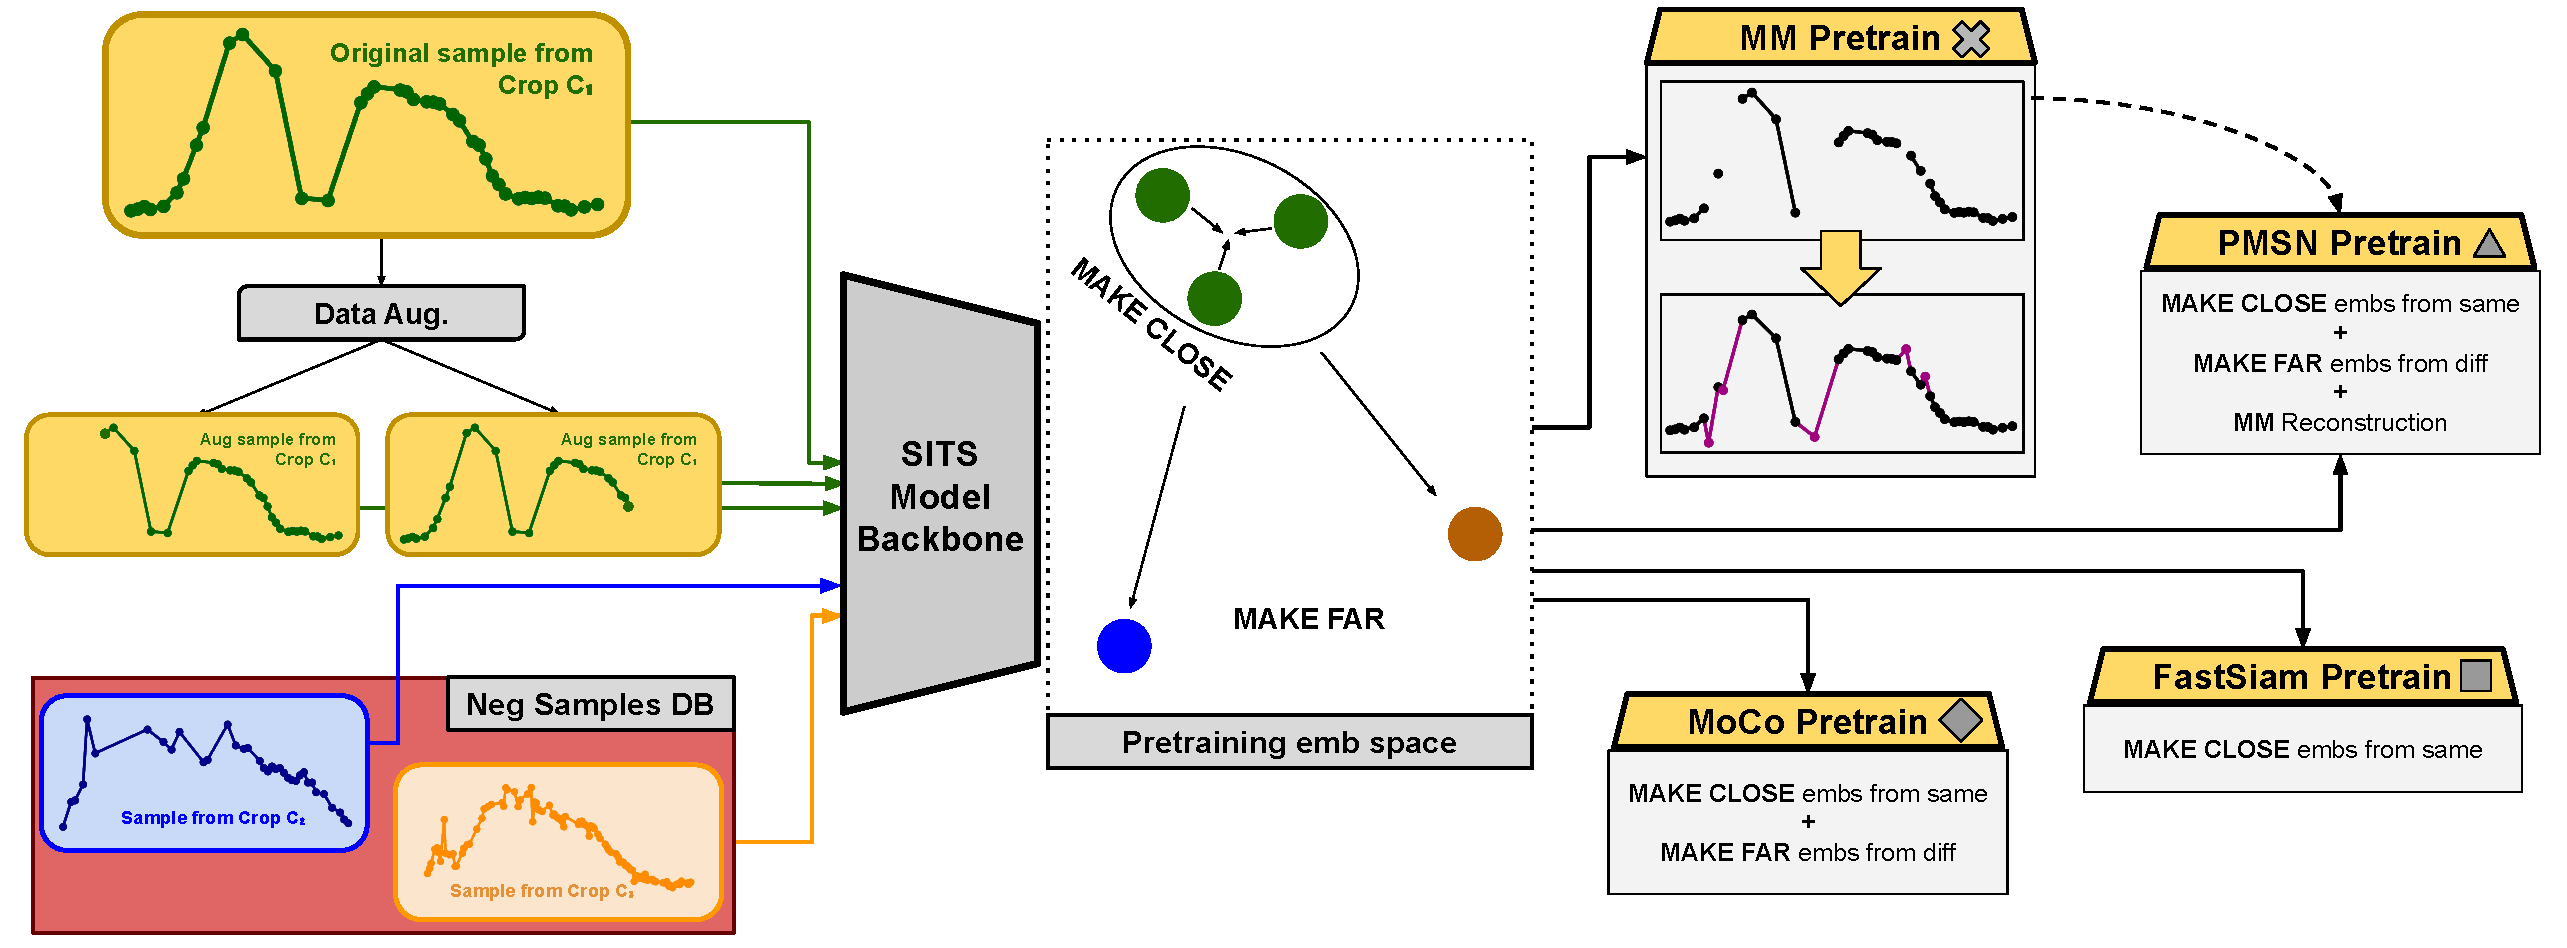
\includegraphics[width=1\linewidth]{figures/6_methodology/meth_ssl.pdf}
\label{fig:meth_ssl}
\end{figure}

To mitigate the scarcity of labeled data from unlabeled \ac{SITS}, this work explores and compares four \ac{SSL} strategies. The selected approaches cover the paradigms of masked modeling/reconstruction, contrastive learning, non-contrastive learning, and hybrid methods.

All strategies use a data augmentation pipeline designed specifically for \ac{SITS} data, in the first paradigm as traditional sample augmentation and the last three to compare augmentations with the data itself and train based on similarities. The transformations applied include: random temporal shift, which simulates variations in planting/harvesting dates; random removal of timestamps, simulating data loss due to clouds or sensor errors; and random swapping of the order of neighboring timestamps. In addition, data normalization is applied consistently.

The first approach evaluated is based on reconstruction via Masked Modeling (MIM). In this configuration, a binary mask is applied to the input, corrupting a percentage of the timestamps in the time series, replacing some timestamps with a token representing the absence of data. The model is trained to predict the values of the original bands of the hidden timestamps, minimizing the Mean Squared Error (MSE) calculated exclusively on the masked elements. This task forces the encoder to learn temporal dependencies and spectral correlations to infer the missing context.

The second strategy employs Momentum Contrast (MoCo), a contrastive method that uses a dynamic dictionary mechanism. The model operates with two encoders: a query encoder, updated via backpropagation, and a key encoder, whose weights are updated via exponential moving average (momentum update) of the query encoder weights. A memory bank is used to store past negative samples, allowing the use of a large number of negatives without the need for excessively large batches. The InfoNCE NT-Xent loss function is used to maximize the similarity between positive view representations while minimizing similarity with negative keys.

The third approach uses FastSiam, a non-contrastive method that does not require the use of negative pairs. The architecture consists of Siamese networks where one of the branches receives an additional prediction head (MLP). To prevent the representation from collapsing into a trivial solution, the stop-gradient operation is applied to the opposite branch. The goal is to maximize the negative cosine similarity between the prediction of one augmented view and the projection of the other view, learning invariance to the applied transformations.

Finally, we evaluate Prior Matching for Siamese Networks (PMSN), a hybrid approach that integrates data masking with prototype-based learning. In this method, an anchor view of the time series is artificially masked, while a target view remains intact, undergoing only standard augmentations. Both representations are projected into a space of trainable prototypes. The loss function seeks to align the probability distribution of the masked anchor with that of the target view on these prototypes, encouraging the model to recognize the semantics of the sample even in the absence of significant parts of the temporal information.

\section{Anomaly Detection and Open Set for SITS}
\label{sec:models_anomaly}

To refine the predictions of SITS classification models, we created an approach focused on the anomaly detection and \ac{OSR} literatures. We propose the \ac{ORDER} method. Although inspired by the GeMOS \ac{OSR} framework~\cite{vendramini2021opening}, \ac{ORDER} substantially advances the methodology by addressing a recurrent challenge in threshold-based methods: the automatic identification of optimal decision boundaries. While \ac{GeMOS} is characterized as a plug-and-play approach that couples GMMs to pretrained neural networks using their embeddings as features, it typically relies on fixed heuristics for rejection. \ac{ORDER} overcomes this limitation by introducing a supervised optimization cycle for hyperparameter optimization and automatic threshold definition. Consequently, the most significant contribution of \ac{ORDER} lies in this fundamental shift in application scope. Unlike the original GeMOS framework, which is primarily designed for \ac{OSR} tasks to identify entirely new and unseen classes, \ac{ORDER} is strictly not intended for open-set scenarios. Instead, its core purpose is the precise discrimination between correct and incorrect predictions within known classes, serving as a robust anomaly detection mechanism to facilitate rigorous dataset cleaning and quality control.

\begin{figure}[ht!]
    \centering
    \caption{Graphical abstract showing the ORDER anomaly detection.}
    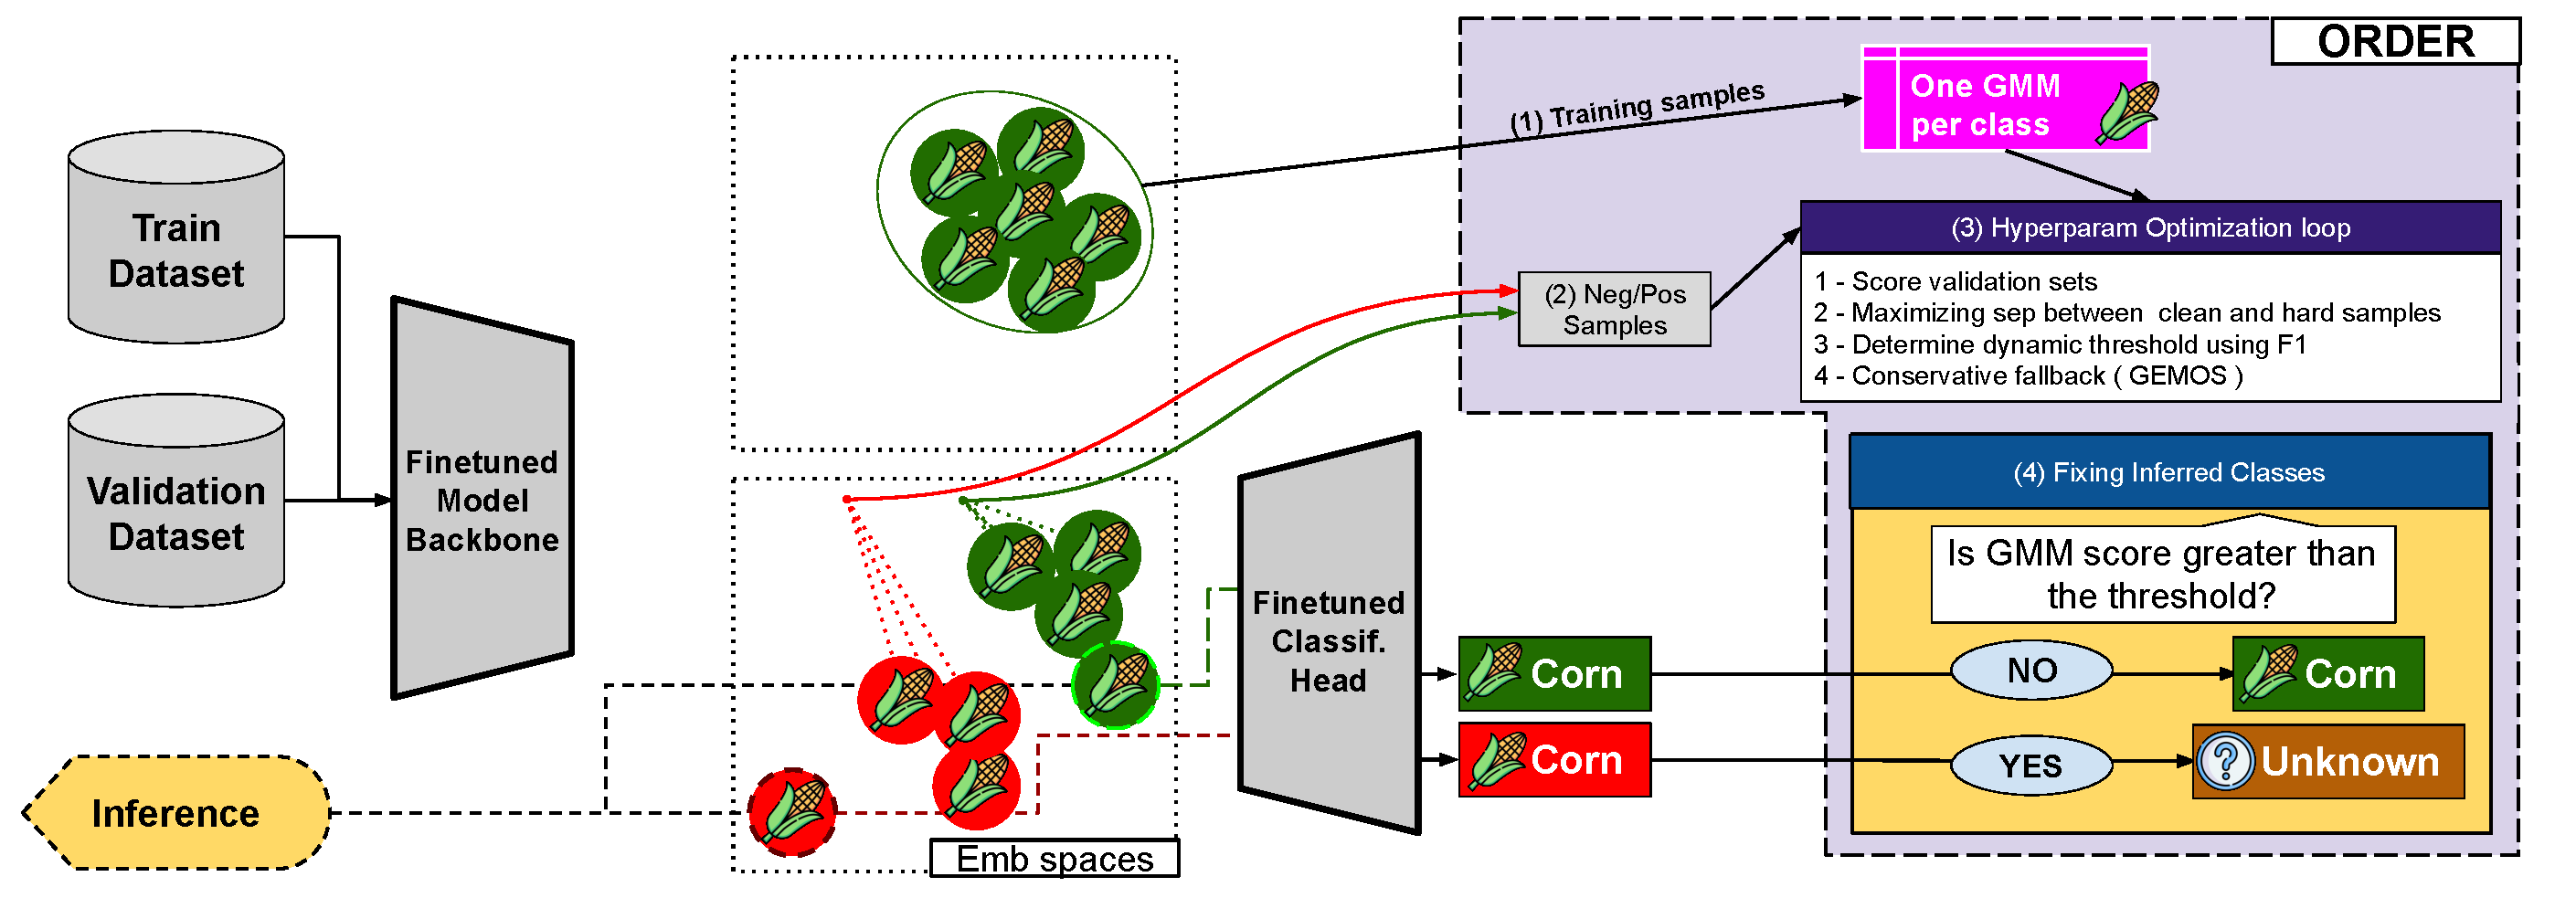
\includegraphics[width=1\linewidth]{figures/6_methodology/meth_models.pdf}
    \label{fig:meth_anomaly}
\end{figure}

As with \ac{GeMOS}, the \ac{ORDER} method uses a dedicated GMM per class, and its main flow iterates over the classes predicted by the base crop classification model. The process begins with feature extraction: in step 1, all correctly classified samples in the training set have their embeddings -  i.e., the intermediate latent representations of the \ac{DL} model - copied to form the training basis for the \ac{GMM} of that class. In step 2, the method processes the validation set, dividing the embeddings into two groups: positive samples (correct classifications) and negative samples (incorrect classifications), which simulate the behavior of hard negatives.

The core contribution of the method lies in step 3, where the stochastic optimization loop of the \ac{GMM} hyperparameters begins. Unlike the standard \ac{GeMOS} approach, which tends to fix the \ac{GMM} hyperparameters (by fixing the number of components), \ac{ORDER} implements an active search for the best configuration through a custom objective function. As detailed in sub-steps 3.1 and 3.2, for each hyperparameter attempt, the candidate model is trained and then used to calculate the log-likelihood of the positive and negative validation groups. The success criterion is not only the fit to the data, but the maximization of the AUC resulting from the separation between these scores. This forces the model to learn a distribution that not only represents the class, but maximizes the distinction between reliable patterns and classifier errors (anomalies).

Solving the threshold definition problem, step 3.3 dynamically establishes the decision boundary. Instead of applying an arbitrary percentile to the training data, the algorithm computes the precision and recall curves based on the validation scores and selects the threshold that maximizes the F1-Score. This strategy adapts the detector's sensitivity to the specific density and dispersion of each class. Finally, sub-step 3.4 acts as a fallback mechanism: if the size of the training set, positive samples, or negative samples is too small for optimization, the method automatically reverts to a conservative configuration, adjusting a \ac{GMM} with one component and setting the cutoff at the 2.5th percentile (basically the standard \ac{GeMOS}, but with values better adjusted for the specific case of \ac{ORDER}), ensuring robustness even in scenarios of very scarce data, or that the model gets the vast majority of samples in the validation sets right or wrong. Although the method has also been tested for OSR, the main focus is anomaly detection for Closed Set.